\documentclass[twocolumn]{article}
\usepackage[utf8]{inputenc}
\usepackage[english]{babel}

\usepackage{xcolor}
\usepackage{blindtext}
\usepackage{graphicx}


\title{A Survey on Interest Flooding Attack (IFA) Countermeasures and Mitigation in Named Data Networking (NDN)}
\author{Abdullah Abumouzah }



\begin{document}

\maketitle

\begin{abstract}

\end{abstract}

\nocite{*}
\section{Introduction}
Information-Centring-Networking is considered to be the next future internet architecture \cite{Ahlgren2012}\\
NDN is one instance of five projects that funded by the United State National Science Foundation (NSF) under the Future Internet Architecture Program (IFA). 

Section II illustrates the NDN architecture. Section III explains the IFA attack. Section IV analyze the current literature. Section V concludes this paper.   

\section{Background}
\subsection{NDN Architecture Overview}
The principle and sturdy design of the NDN architecture is a derivation from the current host-centric network architecture (IP). \cite{Pan2011}. The phenomenal design of the IP internet hourglass involves the thin waist layer which allows the both upper and lower layers to operate independently; it is however the element that causes most of the limitations of the design per se. IP architecture proposed to allow a communication network among endpoints entities that their packets could only be named digitally through the IP address. However, With the dominant growth of the digital media, e-commerce and social network there became a need to use the internet not only for network communication but for content distribution. As per Cisco white paper \cite{Cisco2015}, As per Cisco white paper, on 2014, the content delivery network such as Netflix, Youtube and Akamai had carried about 39\% of the global internet traffic expecting this number to grow up to 62\% on 2019. Just because how the distribution network is more general than the communication network, it is more complex to solve distribution problems with the IP architecture proposals. NDN hourglass architecture Figure.[1] retains the internet hourglass with evolving the thin waist layer to not only containing those problems but also providing secured and more efficient platform. NDN architecture removes the restriction of using the endpoints as the only source to fetch or secure data. In contrast to the communication network, NDN changes the concept of relying on network services to only deliver the packets from a given node address to also being able to fetch data that identified by a given name which serves content distribution schemes.
\begin{figure} [h]
    \centering
    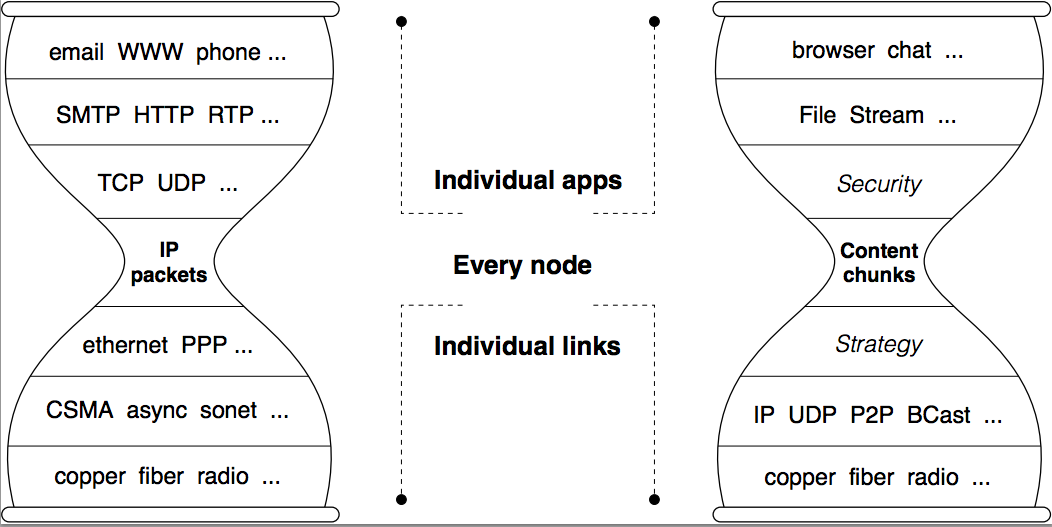
\includegraphics[width=\columnwidth]{hourglass.png}
    \caption{\small NDN Hourglass Architecture}
    \label{fig:my_label}
\end{figure}

NDN by its mean contains significant components that are used for communication: \textbf{\textit{Consumer/Requester}} the one that creates the interest packet for specific content.Provider: the node that has a cached content. \textbf{\textit{Producer}} the node that created and generated the actual content. \textbf{\textit{Interest}} the packet that consumer created to request a specific content. \textbf{\textit{Data}} the packet that forwards the requested content. Data encrypted and signed by the producer and verified by the consumer. In addition, NDN depends in three structures to forward a packet: \textbf{Content Store (CS)} Where data get cached and then it can be self-identified and self-authenticated since it already has the producer's signature if they ever been requested again. Therefore, the cached data could be forwarded to many consumers. Exact matching to the content name (CN) is conducted. \textbf{Pending Interest Tables (PIT)} Creates an entry for each Interest packet the consumer provides; once the corresponding data packet arrives, the router forwards that packet downstream to the requester; if no data packet arrives then the entry expires. Exact matching to the content name (CN) is conducted. \textbf{Forwarding Information Base (FIB)} creates a list of the next destinations and available destinations prefix names. FIB used to forward the interest packet upstream. Longest match to the content name (CN) is conducted.\\
When a consumer creates an interest packet, it first forwards it to the router. [1] Router then searches the CS looking for a matching CN that associated with the interest's CN; if match found, a data packet that has the content and was signed by the provider get forwarded to the consumer. Otherwise, the router looks up in the PIT to find a matching entry. If a matching entry is found then a new interface for the incoming interest packet is added into the interfaces list, and that is known as interest aggregation, so whenever the corresponding data packet is available, it forwards to all the consumers that waiting for the data. If no entry is found for incoming interest packet in the PIT, the interest packet then is passed to the router's FIB where the longest prefix match (LPM) is performed for the CN. FIB creates multiple LPMs for the CN. For example, for /UCCS/CS/6000/lectures CN, the LPMs will be like: /UCCS/, /UCCS/CS/, /UCCS/CS/6000, /UCCS/CS/, /UCCS/CS/6000/lectures. Once a matching FIB entry is found for these LPMs the interest packet is forwarded to the next associated hops and then new PIT entry is created with its incoming interface. Otherwise, the interest packet is flooded and forwarded to all the outgoing interfaces or deleted as per the router's forwarding policies.
When the data packet arrives at the NDN router, the router first look-up for all the corresponding PIT entries and forward the data packet to all interfaces that listed on the list of incoming interfaces. Next, the PIT entry is deleted. In the CS, to serve future requests for the same content, the content is stored based on the local caching policies. However, because of the lifetime of PIT entry policy, an entry will be over and deleted from the list of incoming interfaces, in this case, the data packet will be dropped if no corresponding entry is found.
Below is a detailed explanation for each element of the NDN architecture.


  
It is \cite{zhang2010named}



\subsection{Intrest Forwarding Attack (IFA)}


\bibliographystyle{ieeetr}
\bibliography{Bibliography}
\end{document}
